\chapter{Introduction}
\label{ch:introduction}

\section{Motivation}
\label{sec:intro_motivation}
Efficient transportation systems are fundamental to the vitality and accessibility of university campuses, profoundly impacting student life, operational sustainability, and environmental stewardship \cite{dell2016campus, guido2017sustainable}. For an institution such as the Izmir Institute of Technology (IZTECH), which serves a student population of approximately 5500~\cite{iztech_info} spread across the expansive metropolitan area of Izmir, the logistical complexities are considerable. IZTECH, a key technological university, plays a significant role in the educational and research landscape of the region, making the well-being and accessibility for its students a priority. The challenge of designing an optimized transportation network for IZTECH students is multifaceted. It involves not only managing substantial operational costs related to fuel consumption and vehicle maintenance but also enhancing the daily commute for a large, geographically dispersed student body. The inherent difficulties include optimizing routes with fluctuating demand, developing computationally feasible solutions for a large-scale network, and addressing imperfections in real-world data \cite{kaviani2019smart, saberi2017models}. Therefore, optimizing the student transportation network is crucial for improving student experience, ensuring equitable access to education, and promoting the overall efficiency of the university's operations. This thesis endeavors to address these challenges by systematically applying and rigorously evaluating graph theory principles and advanced clustering algorithms to architect an optimized bus routing system tailored for IZTECH students.

\section{State-of-the-Art}
\label{sec:intro_sota}
The problem of vehicle routing and transportation network optimization has been extensively studied, with a rich body of literature focusing on various methodologies \cite{toth2014vehicle}. Graph theory provides a natural and powerful framework for modeling transportation networks, where locations are represented as vertices and travel segments as edges \cite{tarapata2019graph}. Within this framework, several key areas of research are pertinent to this thesis.

Graph construction techniques are crucial for creating accurate and computationally manageable representations of transportation networks. While complete graphs offer comprehensive connectivity, their $O(N^2)$ complexity is prohibitive for large datasets. Consequently, sparse graph construction methods such as K-Nearest Neighbors (KNN) graphs, Delaunay Triangulation, and Gabriel Graphs are widely adopted. These methods aim to preserve essential connectivity, particularly local spatial relationships, while significantly reducing the number of edges, thereby enhancing computational efficiency (see Chapter~\ref{ch:basics}). The choice of graph representation profoundly influences the subsequent analysis and the quality of the derived solutions.

Once a graph representation is established, clustering algorithms are employed to partition the network into manageable sub-units, which in this context correspond to potential bus routes. Graph clustering, or community detection, seeks to identify groups of vertices that are densely connected internally while being sparsely connected to the rest of the graph. Prominent algorithms in this domain include Spectral Clustering, which utilizes the eigenspectrum of graph Laplacian matrices to find optimal cuts (see Chapter~\ref{ch:basics}). The Leiden algorithm, an improvement over the Louvain method, is another state-of-the-art technique known for its ability to find well-connected communities by optimizing modularity~\cite{leiden}. More advanced methods like Multi-view Anchor Graph-based Clustering (MVAGC) aim to leverage complementary information from different data representations (views) to achieve more robust clustering, often using anchor points to manage complexity (see Chapter~\ref{ch:basics}). The effectiveness of these algorithms can vary depending on the specific characteristics of the network and the chosen graph representation.

Furthermore, outlier detection methods are increasingly recognized as important pre-processing steps in network analysis \cite{lu2020outlier}. Techniques such as K-Nearest Neighbor (KNN) distance-based outlier detection help identify and handle anomalous data points that could otherwise skew clustering results and lead to inefficient or impractical routes~\cite{knn_outlier}. Shortest path algorithms, with Dijkstra's algorithm being a cornerstone, are then used to determine the optimal travel path within each identified cluster or route (see Chapter~\ref{ch:basics}). This thesis builds upon these state-of-the-art techniques, tailoring and evaluating them for the specific problem of university student transportation.

\section{Problem Statement}
\label{sec:intro_problems}
Optimizing the student transportation network for IZTECH presents several distinct challenges that this thesis aims to address:

\begin{itemize}
    \item \textbf{Isolated Student Locations:} A significant number of students may reside in locations that are geographically distant from main student population centers or from each other. These "isolated vertices" complicate route planning, as servicing them can lead to excessively long routes or underutilized buses, thereby increasing per-student transportation costs. Identifying and efficiently integrating or managing these outliers is crucial.
    \begin{figure}[!htbp]
        \centering
        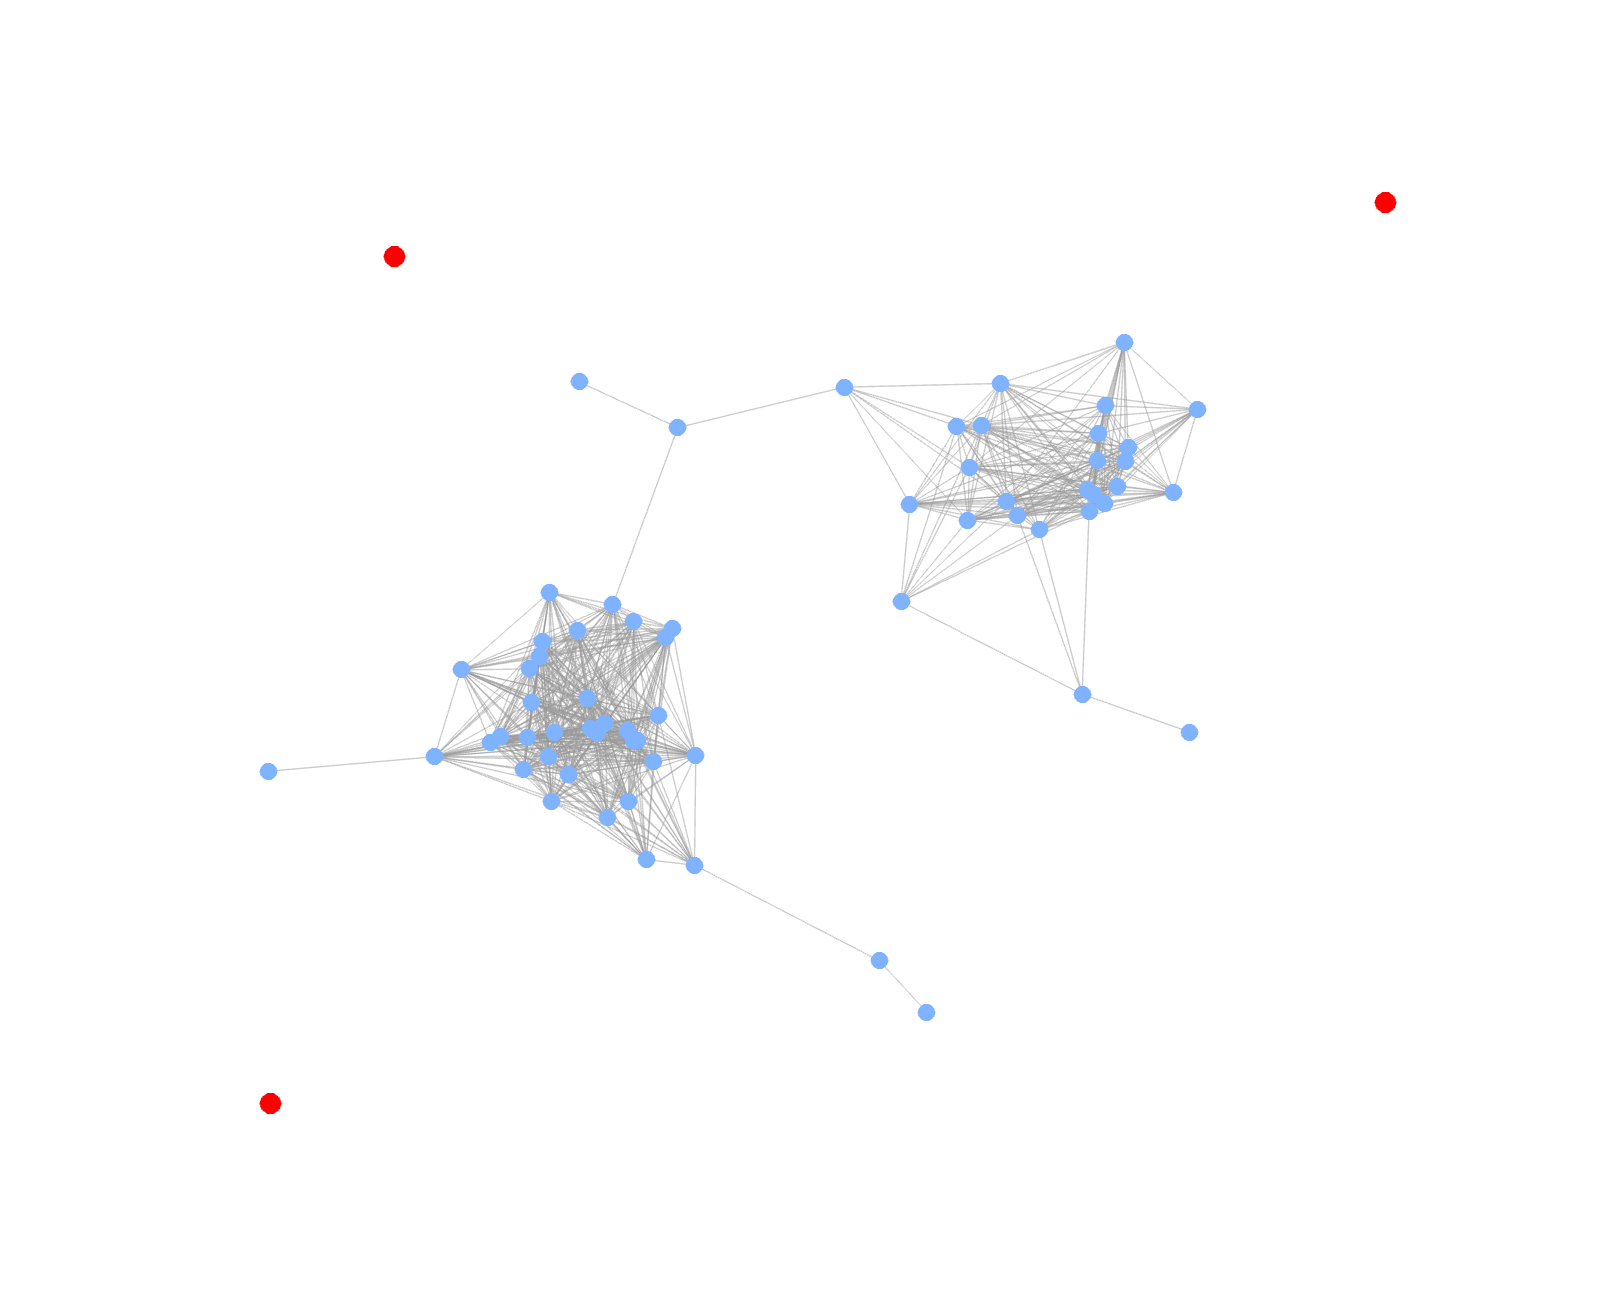
\includegraphics[width=0.9\textwidth]{img/robustness_problem.png}
        \caption{Illustration of the 'Isolated Student Locations' problem. Distant students (highlighted, e.g., in red) can necessitate disproportionately long and costly detours if included in standard routes, impacting overall efficiency.}
        \label{fig:problem_isolated_students}
    \end{figure}

    \item \textbf{Limited Service Capacity:} The university's bus fleet has specific capacity constraints. Each vehicle can typically accommodate a minimum of 10 and a maximum of 50 students. Clustering algorithms and route planning must strictly adhere to these capacity limits to ensure both operational feasibility and cost-effectiveness. Generating routes that are either too small (underutilized) or too large (exceeding capacity) is a key problem.

    \item \textbf{Fuel Consumption and Budget Limitations:} Fuel costs constitute a major portion of the transportation budget. Minimizing total distance traveled by all buses is a primary objective to reduce fuel consumption and operate within budgetary constraints. This necessitates the design of compact and efficient routes.

    \item \textbf{Large Number of Students:} With approximately 2000 students requiring transportation across a large metropolitan area, the scale of the network is substantial. This large number of nodes leads to high computational complexity for many graph algorithms, especially those involving dense matrix operations or exhaustive searches. Scalable and efficient algorithms are therefore essential.
    \begin{figure}[!htbp]
        \centering
        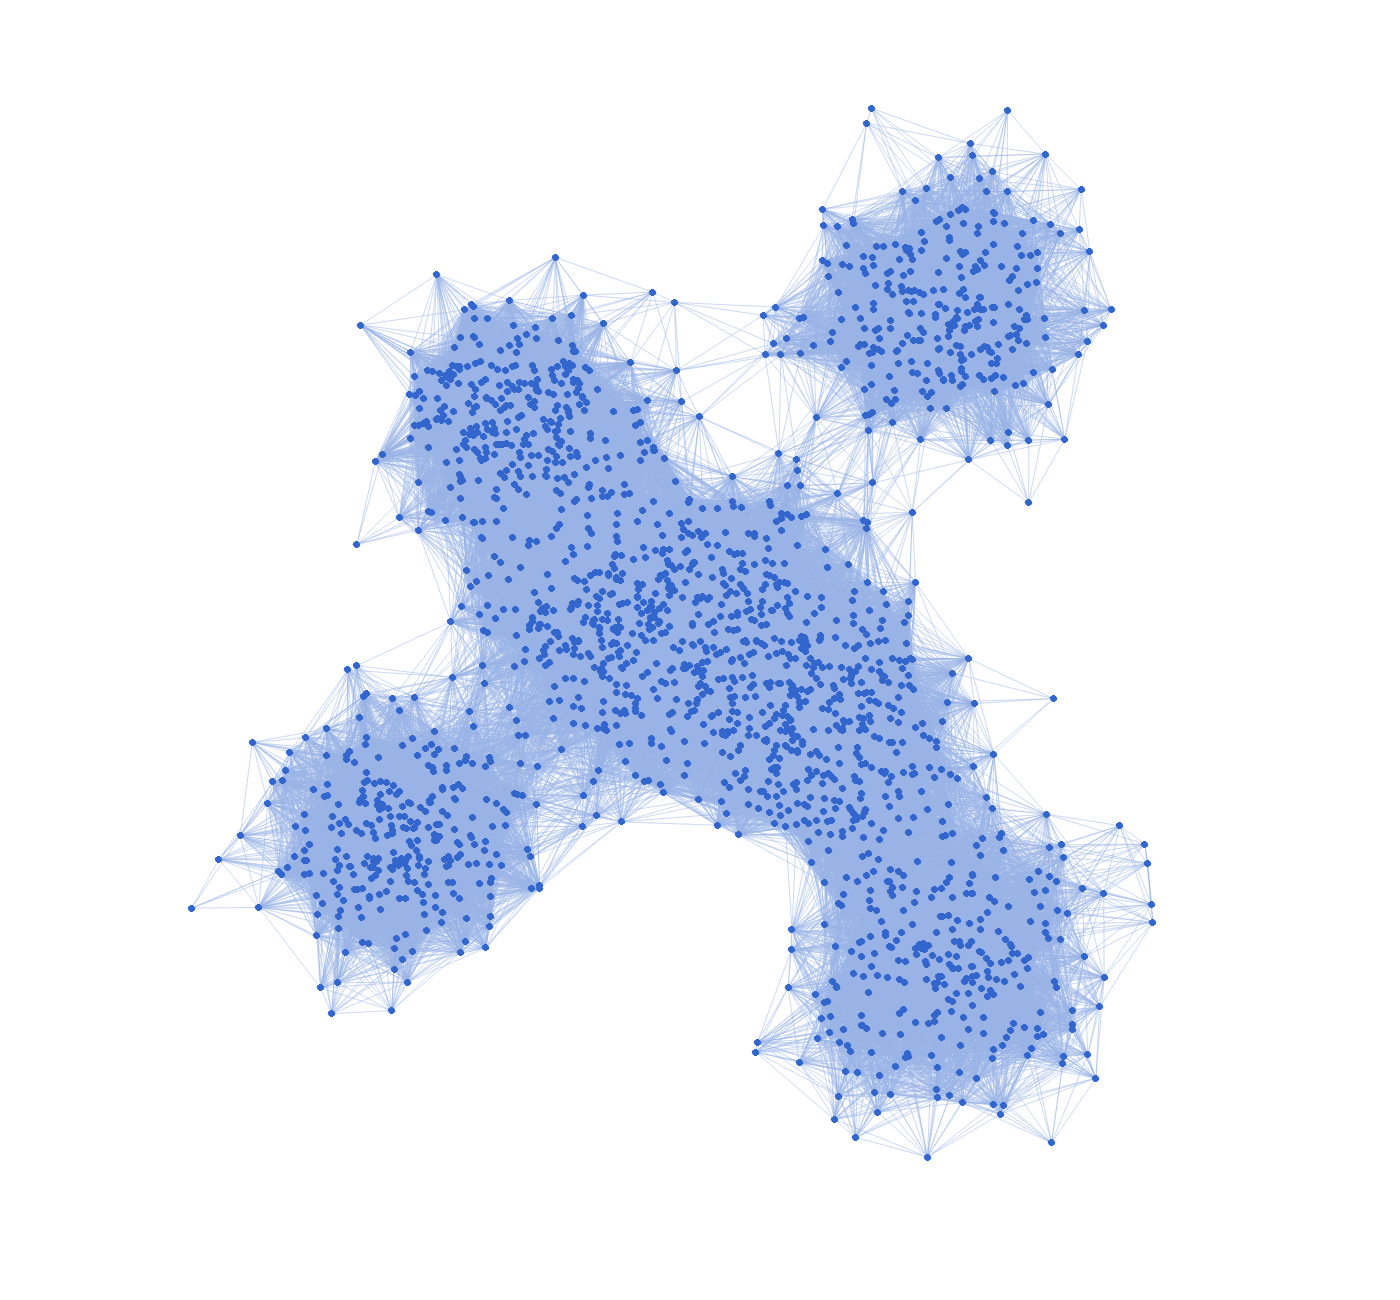
\includegraphics[width=0.7\textwidth]{img/large_scale_students.png}
        \caption{Representing the 'Large Number of Students' problem. The sheer volume and density of approximately 2000 student locations (nodes in the network), as illustrated here, significantly increase the computational complexity of finding optimal routing solutions.}
        \label{fig:problem_large_scale}
    \end{figure}

    \item \textbf{Non-Static Address Information:} While this thesis utilizes a synthetically generated dataset based on current general population distribution, in a real-world scenario, student address information can be non-static, changing semester by semester. An effective system should ideally be adaptable to such changes, although this aspect is more related to the operationalization than the core algorithmic design focused on here. The current work focuses on optimizing for a given snapshot of student locations.
\end{itemize}
Addressing these interconnected problems requires a holistic approach that balances cost, efficiency, service quality, and computational tractability.

\section{Our Proposed Solution}
\label{sec:intro_solution}
This thesis puts forth a solution focused on three primary contributions to optimize the IZTECH student transportation network, each addressing specific challenges outlined in Section~\ref{sec:intro_problems}:

\begin{enumerate}
    \item \textbf{Determining the necessary number of services and alternative solutions:} A key goal is to ascertain the optimal fleet size and explore various route configurations, thereby addressing the issues of Limited Service Capacity by ensuring routes adhere to the 10-50 student limit, and tackling the Large Number of Students by breaking the problem into manageable parts. Our approach achieves this by applying different graph clustering algorithms to partition the student population into potential bus routes, as detailed in Section~\ref{subsec:clustering_sparse}. By comparatively analyzing the outcomes—considering factors like the total number of routes, overall cost (which relates to Fuel Consumption and Budget Limitations), and adherence to capacity constraints—we identify a range of viable solutions and pinpoint the most efficient configurations \cite{zhang2018data}.
    
    \item \textbf{Efficiently determining service routes:} This refers to the development of computationally tractable and cost-effective methods for defining the actual paths for each bus service, directly targeting Fuel Consumption and Budget Limitations and the challenge of a Large Number of Students. We begin by employing sparse graph representations (specifically Delaunay Triangulation, Gabriel Graphs, and K-Nearest Neighbors Graphs) of the student network, as described in Section~\ref{subsec:sparse_graph}, which significantly reduces computational complexity. Once students are grouped via clustering, Dijkstra\'s algorithm (Section~\ref{sec:shortest_path}) is utilized to calculate the shortest path connecting students within each group, further minimizing travel distances and defining optimized service routes.
    
    \item \textbf{Ensuring robustness for isolated addresses:} This contribution directly tackles the problem of Isolated Student Locations, where students residing in geographically distant areas could lead to significant inefficiencies. Our solution incorporates a K-Nearest Neighbor (KNN) distance-based outlier detection method as a crucial preprocessing step (Section~\ref{subsec:knn_outlier_application}). This method identifies students whose locations are statistical outliers, allowing them to be handled separately or excluded. This not only improves route compactness, thereby contributing to reducing Fuel Consumption and Budget Limitations, thus enhancing the practicality and cost-effectiveness of the overall transportation plan.
\end{enumerate}

The comprehensive methodology to realize these contributions integrates these specific techniques. It begins with constructing an appropriate graph model of the student network using one of the selected sparse graph methods (Section~\ref{subsec:sparse_graph}). This is followed by the KNN distance-based outlier detection for data refinement (Section~\ref{subsec:knn_outlier_application}). Subsequently, a comparative evaluation of diverse graph clustering algorithms (Spectral Clustering, Leiden Algorithm, and Multi-view Anchor Graph-based Clustering), detailed in Section~\ref{subsec:clustering_sparse}, is performed to partition the students into capacity-constrained routes. Finally, Dijkstra's algorithm (Section~\ref{sec:shortest_path}) determines the optimal path for each route. The interplay between these components—graph construction, outlier detection, and clustering—is analyzed in detail to identify the most effective combination for the IZTECH student transportation problem.

\section{Thesis Overview}
\label{sec:intro_overview}
This thesis is structured to systematically present the research methodology, experimental evaluation, and findings.
\begin{itemize}
    \item \textbf{Chapter~\ref{ch:introduction}} (this chapter) outlines the motivation, discusses the state-of-the-art, defines the problem scope, introduces our proposed solution, and provides this overview of the thesis structure.
    \item \textbf{Chapter~\ref{ch:basics}} provides the necessary theoretical background. It covers fundamental concepts in graph theory, details various graph construction methods and the significance of sparsity, explains the principles behind the selected graph clustering algorithms (Spectral Clustering, Leiden Algorithm, MVAGC), discusses shortest path computation (Dijkstra's algorithm), and introduces the K-Nearest Neighbor distance-based outlier detection technique.
    \item \textbf{Chapter~\ref{ch:method}} details the specific methodologies employed in this research. This includes the generation of the synthetic student dataset, the practical implementation of the different graph construction techniques (Complete, Delaunay, Gabriel, KNN), the adaptation and application of the clustering algorithms to these graphs with capacity constraints, the implementation of the outlier detection process, and the method for shortest path calculation within clusters.
    \item \textbf{Chapter~\ref{ch:experiments}} presents a comprehensive experimental evaluation of the proposed methods. It compares the performance of different combinations of graph construction techniques and clustering algorithms, both with and without outlier detection. The evaluation is based on key metrics including total transportation cost, number of routes, average route length, average cluster size, and computational time. The results are analyzed to identify the most effective and efficient approaches.
    \item \textbf{Chapter~\ref{ch:conclusions}} summarizes the key findings of the research, discusses the main contributions of the thesis to the field of transportation network optimization, and suggests potential avenues for future work, including methodological advancements and practical implementations.
    \item The \textbf{Appendix} may contain supplementary materials, such as detailed experimental results or pseudocode for algorithms not fully detailed in the main text.
\end{itemize}
Through this structured approach, the thesis aims to provide a clear and thorough investigation into optimizing university student transportation networks using graph-based methods.




